\subsection{MTCNN}
Multi-task Cascaded Convolutional Networks, sometimes known as MTCNN, is a well-liked face identification technique that is frequently applied in computer vision applications. It is particularly made to locate and locate faces accurately in photos. The MTCNN performs face identification, alignment, and landmark localization using three cascaded networks.

The "Proposal Network" (P-Net), the first stage of MTCNN, creates a set of candidate bounding boxes that could include faces. The second step, known as the "Refine Network" (R-Net), which use regression and classification to increase the precision of the bounding box predictions, refines these candidate boxes. The third step, referred to as the "Output Network" (O-Net), completes additional refining and localisation of face landmarks.
\begin{figure}[h]
    \centering
    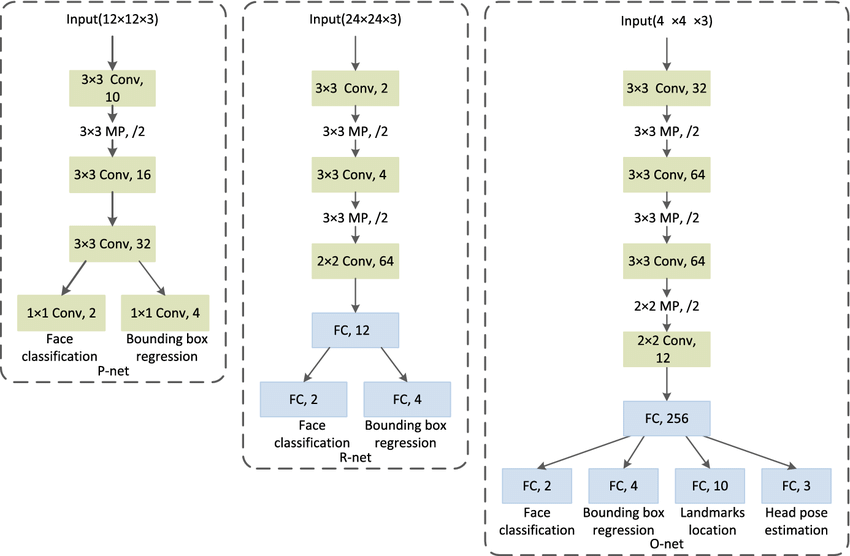
\includegraphics[width= 5in ]{img/MTCNN.png}
    \caption{MTCNN Architecture}
\end{figure}